\documentclass{standalone}
\usepackage{tikz}
\usetikzlibrary{decorations.pathreplacing,decorations.pathmorphing}
\usetikzlibrary{fit,quotes}
\usepackage{yquant, braket}

\begin{document}

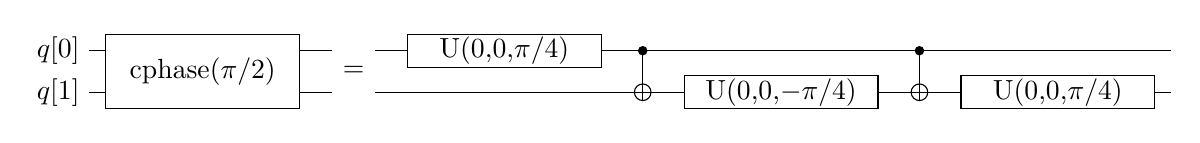
\begin{tikzpicture}[scale=1.000000,x=1pt,y=1pt]
\filldraw[color=white] (0.000000, -7.500000) rectangle (391.000000, 22.500000);
% Drawing wires
% Line 1: q0 W q[0]
\draw[color=black] (0.000000,15.000000) -- (391.000000,15.000000);
\draw[color=black] (0.000000,15.000000) node[left] {$q[0]$};
% Line 2: q1 W q[1]
\draw[color=black] (0.000000,0.000000) -- (391.000000,0.000000);
\draw[color=black] (0.000000,0.000000) node[left] {$q[1]$};
% Done with wires; drawing gates
% Line 3: q0 q1 G {cphase$\left(\pi/2\right)$} width=70
\draw (41.000000,15.000000) -- (41.000000,0.000000);
\begin{scope}
\draw[fill=white] (41.000000, 7.500000) +(-45.000000:49.497475pt and 19.091883pt) -- +(45.000000:49.497475pt and 19.091883pt) -- +(135.000000:49.497475pt and 19.091883pt) -- +(225.000000:49.497475pt and 19.091883pt) -- cycle;
\clip (41.000000, 7.500000) +(-45.000000:49.497475pt and 19.091883pt) -- +(45.000000:49.497475pt and 19.091883pt) -- +(135.000000:49.497475pt and 19.091883pt) -- +(225.000000:49.497475pt and 19.091883pt) -- cycle;
\draw (41.000000, 7.500000) node {{cphase$\left(\pi/2\right)$}};
\end{scope}
% Line 4: =
\draw[fill=white,color=white] (88.000000, -6.000000) rectangle (103.000000, 21.000000);
\draw (95.500000, 7.500000) node {$=$};
% Line 5: q0 G {U(0,0,$\pi/4$)} width=70
\begin{scope}
\draw[fill=white] (150.000000, 15.000000) +(-45.000000:49.497475pt and 8.485281pt) -- +(45.000000:49.497475pt and 8.485281pt) -- +(135.000000:49.497475pt and 8.485281pt) -- +(225.000000:49.497475pt and 8.485281pt) -- cycle;
\clip (150.000000, 15.000000) +(-45.000000:49.497475pt and 8.485281pt) -- +(45.000000:49.497475pt and 8.485281pt) -- +(135.000000:49.497475pt and 8.485281pt) -- +(225.000000:49.497475pt and 8.485281pt) -- cycle;
\draw (150.000000, 15.000000) node {{U(0,0,$\pi/4$)}};
\end{scope}
% Line 6: q0 +q1
\draw (200.000000,15.000000) -- (200.000000,0.000000);
\filldraw (200.000000, 15.000000) circle(1.500000pt);
\begin{scope}
\draw[fill=white] (200.000000, 0.000000) circle(3.000000pt);
\clip (200.000000, 0.000000) circle(3.000000pt);
\draw (197.000000, 0.000000) -- (203.000000, 0.000000);
\draw (200.000000, -3.000000) -- (200.000000, 3.000000);
\end{scope}
% Line 7: q1 G {U(0,0,$-\pi/4$)} width=70
\begin{scope}
\draw[fill=white] (250.000000, -0.000000) +(-45.000000:49.497475pt and 8.485281pt) -- +(45.000000:49.497475pt and 8.485281pt) -- +(135.000000:49.497475pt and 8.485281pt) -- +(225.000000:49.497475pt and 8.485281pt) -- cycle;
\clip (250.000000, -0.000000) +(-45.000000:49.497475pt and 8.485281pt) -- +(45.000000:49.497475pt and 8.485281pt) -- +(135.000000:49.497475pt and 8.485281pt) -- +(225.000000:49.497475pt and 8.485281pt) -- cycle;
\draw (250.000000, -0.000000) node {{U(0,0,$-\pi/4$)}};
\end{scope}
% Line 8: q0 +q1
\draw (300.000000,15.000000) -- (300.000000,0.000000);
\filldraw (300.000000, 15.000000) circle(1.500000pt);
\begin{scope}
\draw[fill=white] (300.000000, 0.000000) circle(3.000000pt);
\clip (300.000000, 0.000000) circle(3.000000pt);
\draw (297.000000, 0.000000) -- (303.000000, 0.000000);
\draw (300.000000, -3.000000) -- (300.000000, 3.000000);
\end{scope}
% Line 9: q1 G {U(0,0,$\pi/4$)} width=70
\begin{scope}
\draw[fill=white] (350.000000, -0.000000) +(-45.000000:49.497475pt and 8.485281pt) -- +(45.000000:49.497475pt and 8.485281pt) -- +(135.000000:49.497475pt and 8.485281pt) -- +(225.000000:49.497475pt and 8.485281pt) -- cycle;
\clip (350.000000, -0.000000) +(-45.000000:49.497475pt and 8.485281pt) -- +(45.000000:49.497475pt and 8.485281pt) -- +(135.000000:49.497475pt and 8.485281pt) -- +(225.000000:49.497475pt and 8.485281pt) -- cycle;
\draw (350.000000, -0.000000) node {{U(0,0,$\pi/4$)}};
\end{scope}
% Done with gates; drawing ending labels
% Done with ending labels; drawing cut lines and comments
% Done with comments
\end{tikzpicture}
\end{document}
